\documentclass[11pt,a4paper]{article}
\usepackage[T1]{fontenc}
\usepackage[margin=2.3cm]{geometry}
\usepackage{amsmath,amssymb}
\usepackage{graphicx}
\usepackage[dvipsnames]{xcolor}
\usepackage{enumitem}
\usepackage[colorlinks=true,linkcolor=blue,urlcolor=blue]{hyperref}
\setlength{\parskip}{0.6em}
\setlength{\parindent}{0pt}
\begin{document}

\begin{center}{\LARGE\bfseries opensorting}\\[0.4em]{\large Race sorting algorithms and count every comparison, swap and second, in three sessions.}\\[0.2em]\small PAN IIT OSS explainer \textbullet{} secondary school to diploma / undergraduate (levels 3-5)\end{center}

\section*{Why this exists}
Every program that handles data sorts it sooner or later. Two correct sorting programs can differ by a factor of thousands in the number of steps. This explainer shows how to count steps, fit growth curves and choose a method, using only Python.

\section*{The end goal}
Compare sorting algorithms by swaps, comparisons and time. The end goal is to compare sorting algorithms by swaps, comparisons and time, and to explain why a more efficient algorithm can perform much better on a large dataset even when both produce the same answer.

\section*{How the three sessions build up}
\begin{enumerate}[nosep]
\item \textbf{Session 1: Sorting cards by hand is an algorithm} (Level 1, conceptual interactive model, 60 min).
\item \textbf{Session 2: Five algorithms, one step counter} (Level 2, mathematical engineering model, 80 min).
\item \textbf{Session 3: Measuring growth, failure cases and choosing a method} (Level 3, simulation and validation, 90 min).
\end{enumerate}

\section{Session 1: Sorting cards by hand is an algorithm}

\subsection*{A. Real-world problem}
You are dealt five cards and put them in order without thinking about it. A computer cannot think, so it needs the rules written down exactly. Two rule sets are easy to follow: look at neighbours and swap them if they are in the wrong order (bubble sort), or take each new card and slide it left until it fits (insertion sort). Both give the same sorted row. Do they take the same number of steps? And does it depend on how mixed up the cards were at the start?

\subsection*{B. Concept and theory}
A row of n cards is sorted when every card is not bigger than the card to its right. A comparison looks at two cards. A swap exchanges two neighbours. Bubble sort walks along the row swapping neighbours that are in the wrong order, so the biggest card bubbles to the end; it repeats on the shorter row that is left, and stops early after a walk with no swap. Insertion sort takes the next card and slides it left one place at a time past every bigger card. An inversion is a pair of cards where the bigger one is to the left of the smaller one. A swap of two neighbours removes exactly one inversion, so both methods use as many swaps as there are inversions at the start. A sorted row has 0 inversions; a reversed row of n cards has n(n-1)/2, the most possible.

\begin{itemize}[nosep]
\item n: number of cards in the row (cards)
\item k: number of leading cards that start reversed (cards)
\item comparisons: times two cards were looked at (count)
\item swaps: times two neighbours were exchanged (count)
\item inversions: pairs of cards in the wrong order (count)
\end{itemize}

\begin{equation*}
\text{swaps}=\text{inversions}=\#\{(i,j):\ i<j,\ a_i>a_j\}
\end{equation*}

\begin{equation*}
\text{inversions of a reversed row}=\frac{n(n-1)}{2}
\end{equation*}

\begin{equation*}
\text{bubble sort on a sorted row: } n-1 \text{ comparisons, } 0 \text{ swaps}
\end{equation*}

\begin{center}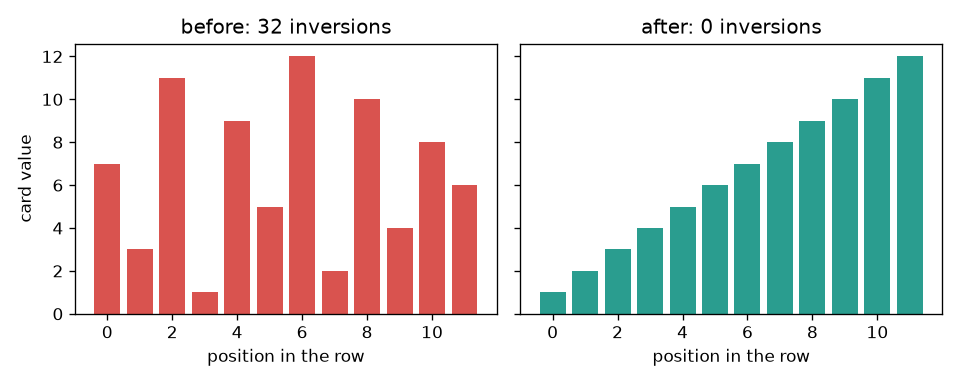
\includegraphics[width=0.85\linewidth]{figures/s01_bars_before_after.png}\\\small A row of 12 cards as bars: 32 pairs in the wrong order before, none after.\end{center}

\subsection*{E. Worked example}
Sort the cards 5 2 4 1 3 with bubble sort and with insertion sort. Count comparisons and swaps for each, and check against the number of pairs in the wrong order.
\begin{enumerate}[nosep]
\item Pairs in the wrong order: (5,2), (5,4), (5,1), (5,3), (2,1), (4,1), (4,3), so 7 inversions. Both methods must use 7 swaps.
\item Bubble walk 1 compares (5,2) swap, (5,4) swap, (5,1) swap, (5,3) swap: 4 comparisons, 4 swaps, row 2 4 1 3 5.
\item Bubble walk 2 compares (2,4) no swap, (4,1) swap, (4,3) swap: 3 comparisons, 2 swaps, row 2 1 3 4 5. Walk 3 compares (2,1) swap, (2,3) no swap: 2 comparisons, 1 swap, row 1 2 3 4 5. Walk 4 compares (1,2): 1 comparison, no swap, so it stops. Total 4 + 3 + 2 + 1 = 10 comparisons and 4 + 2 + 1 = 7 swaps.
\item Insertion sort: the 2 passes 1 comparison (swap); the 4 needs 2 comparisons (one swap); the 1 slides past 5, 4 and 2 (3 comparisons, 3 swaps); the 3 slides past 5 and 4 and stops at 2 (3 comparisons, 2 swaps). Total 1 + 2 + 3 + 3 = 9 comparisons and 1 + 1 + 3 + 2 = 7 swaps.
\end{enumerate}
\textbf{Answer.} Bubble sort: 10 comparisons and 7 swaps. Insertion sort: 9 comparisons and 7 swaps. Both swap counts equal the 7 inversions.

\subsection*{F. Questions}
\begin{enumerate}[nosep]
\item \textbf{Conceptual.} Why do bubble sort and insertion sort need exactly the same number of swaps for the cards 5 2 4 1 3, even though they work differently?
\item \textbf{Numerical.} A row of 30 cards is completely reversed (30 down to 1). How many comparisons and swaps does insertion sort need? Check your answer with a formula.
\item \textbf{Graph and simulation interpretation.} In the steps graph for 30 cards, at k = 10 (the first 10 cards reversed), which method needs fewer comparisons and by how many? How many swaps do they need?
\item \textbf{Design and optimisation challenge.} Design: a teacher hands you 30 cards that are sorted except that the first 20 are in reverse order. You must pick bubble sort or insertion sort and tell the class how many comparisons to expect. Which do you pick and why? What would you pick if the cards were already sorted?
\end{enumerate}

\section{Session 2: Five algorithms, one step counter}

\subsection*{A. Real-world problem}
A shop has 1,000,000 orders to put in date order. Two programs give exactly the same sorted answer, yet one finishes in a fraction of a second and the other keeps the computer busy for minutes. Why can a more efficient algorithm perform so much better on a large dataset even when both give the same answer? The answer is the number of steps each one takes, and how fast that number grows when the list grows.

\subsection*{B. Concept and theory}
We count steps instead of seconds, because seconds depend on the computer. Bubble, selection and insertion sort compare many pairs of items: in the worst case about n(n-1)/2 comparisons, which grows with the square of n. Merge sort splits the list in halves, sorts each half and merges them; there are about log2 n levels of splitting and each level touches n items, so about n log2 n steps. Quicksort picks a pivot and splits the items into smaller and larger ones; with good pivots it also takes about n log2 n steps. For n = 1000 items the two formulas give 499,500 and 9,966, and the gap widens as n grows. Insertion sort is special: its work is about n - 1 comparisons plus the number of inversions, so it is nearly linear on nearly sorted data. A sort is stable if items with equal keys stay in their original order.

\begin{itemize}[nosep]
\item n: number of items to sort (items)
\item C: number of comparisons (count)
\item M: number of moves (swaps, shifts or copies) (count)
\item log2 n: how many times n can be halved until 1 remains (no unit)
\item key: the value the items are sorted by (any comparable value)
\end{itemize}

\begin{equation*}
C_{\text{insertion}}(\text{reversed list})=M_{\text{insertion}}=\frac{n(n-1)}{2}
\end{equation*}

\begin{equation*}
\frac{n}{2}\log_2 n\ \le\ C_{\text{merge}}\ \le\ n\log_2 n-n+1
\end{equation*}

\begin{equation*}
\frac{n(n-1)/2}{n\log_2 n}\approx\frac{n}{2\log_2 n}
\end{equation*}

\begin{equation*}
C_{\text{insertion}}=M_{\text{insertion}}+(\text{items that do not slide all the way left})\ \le\ \text{inversions}+n-1
\end{equation*}

\begin{center}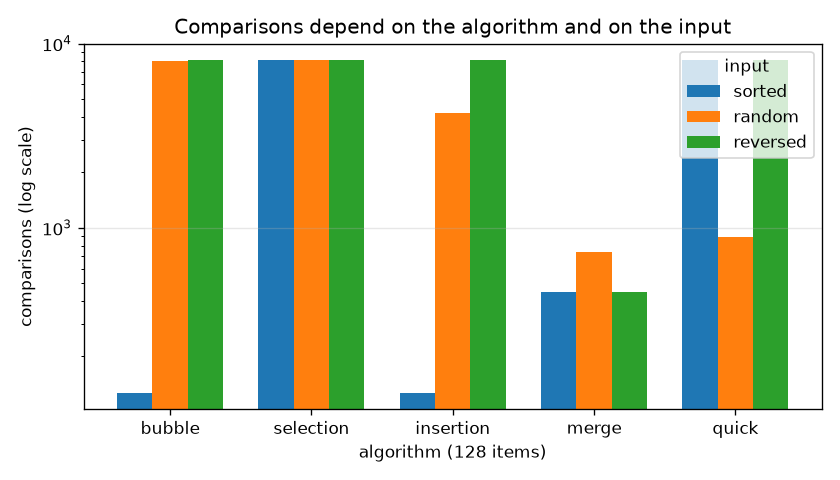
\includegraphics[width=0.85\linewidth]{figures/s02_comparisons_by_input.png}\\\small Comparisons of the five methods on sorted, random and reversed lists of 128 items (log scale).\end{center}

\subsection*{E. Worked example}
A list has n = 1,000,000 items. Compare n(n-1)/2 comparisons with n log2 n comparisons. How many times more is the first? How long does each take at 1 billion steps per second?
\begin{enumerate}[nosep]
\item n(n-1)/2 = 1,000,000 * 999,999 / 2 = 499,999,500,000 comparisons, about 5.0e11.
\item log2 1,000,000 = 19.93, so n log2 n = 19,931,569 comparisons, about 2.0e7.
\item Ratio = 499,999,500,000 / 19,931,569 = 25,086, about 25,000 times more.
\item At 1e9 steps per second: 499,999,500,000 / 1e9 = 500 seconds, about 8 minutes; 19,931,569 / 1e9 = 0.0199 seconds, about 0.02 seconds.
\end{enumerate}
\textbf{Answer.} About 5.0e11 versus 2.0e7 comparisons, a ratio of about 25,086, which is 500 seconds against 0.02 seconds at 1e9 steps per second.

\subsection*{F. Questions}
\begin{enumerate}[nosep]
\item \textbf{Conceptual.} Two programs sort the same 1,000,000 records and give identical answers. Why can the more efficient algorithm be hugely faster on this large dataset, even though both are correct?
\item \textbf{Numerical.} Predict how many comparisons insertion sort needs on a reversed list of 100 items, and how many item shifts. Then say what the answer would be for a sorted list of 100 items.
\item \textbf{Graph and simulation interpretation.} In the bar figure for 128 items, selection sort has the same height for sorted, random and reversed input, while insertion sort does not. Explain this, and give the numbers for n = 1000 sorted and reversed.
\item \textbf{Design and optimisation challenge.} Design: a log file of 1000 lines is nearly sorted by time, with 10 neighbouring lines swapped at random. Choose between insertion sort, merge sort and quick sort (first item as pivot) and justify your choice with step counts.
\end{enumerate}

\section{Session 3: Measuring growth, failure cases and choosing a method}

\subsection*{A. Real-world problem}
A textbook says 'merge sort is n log n'. A colleague says 'quicksort is faster'. A third says 'Python's sorted() beats both'. Who is right depends on your data. To decide, you measure: count operations over a range of sizes, fit growth curves, try sorted, reversed, duplicate-heavy and nearly sorted inputs, look for the input that breaks each method, and justify your choice. This is how engineers choose a sorting method for a real data feed.

\subsection*{B. Concept and theory}
If the cost grows like a power, cost = a * n\textasciicircum{}p, then taking logarithms gives log(cost) = log(a) + p log(n), a straight line whose slope is the exponent p. We fit that line to operation counts measured for several sizes. We expect slope about 2 for bubble, selection and insertion sort. For n log n the local slope is 1 + 1/ln n, a little above 1 (about 1.14 near n = 1600), so we expect values such as 1.1 to 1.2, not exactly 1. Quicksort with the first item as pivot on sorted input splits off one item at a time, so it does n(n-1)/2 comparisons and recurses n - 1 levels deep; choosing the pivot at random or as the median of the first, middle and last item avoids that case, but no simple rule is safe for every pattern. A hybrid merge sort sorts small pieces with insertion sort, which has less overhead on tiny lists. Merge sort needs extra space of order n for the merged lists; insertion, selection and bubble sort need almost none. Python's sorted() uses Timsort, which is known to find runs that are already ascending or descending: on presorted input it needs only n - 1 comparisons. We check all of this by measurement, with counts for the main claims and wall-clock times only as illustration.

\begin{itemize}[nosep]
\item n: number of items (items)
\item p: growth exponent: slope of log cost against log n (no unit)
\item a: constant factor of the cost (steps)
\item cutoff: piece size at or below which the hybrid uses insertion sort (items)
\item depth: number of nested pieces in quicksort's recursion (levels)
\item k: number of random swaps applied to a sorted list (swaps)
\end{itemize}

\begin{equation*}
\text{cost}=a\,n^{p}\ \Longrightarrow\ \log(\text{cost})=\log a+p\,\log n
\end{equation*}

\begin{equation*}
p=\frac{d\ln(n\ln n)}{d\ln n}=1+\frac{1}{\ln n}
\end{equation*}

\begin{equation*}
C_{\text{quick, first pivot, sorted input}}=\frac{n(n-1)}{2},\qquad \text{depth}=n-1
\end{equation*}

\begin{equation*}
C_{\text{timsort}}(\text{presorted})=n-1
\end{equation*}

\begin{center}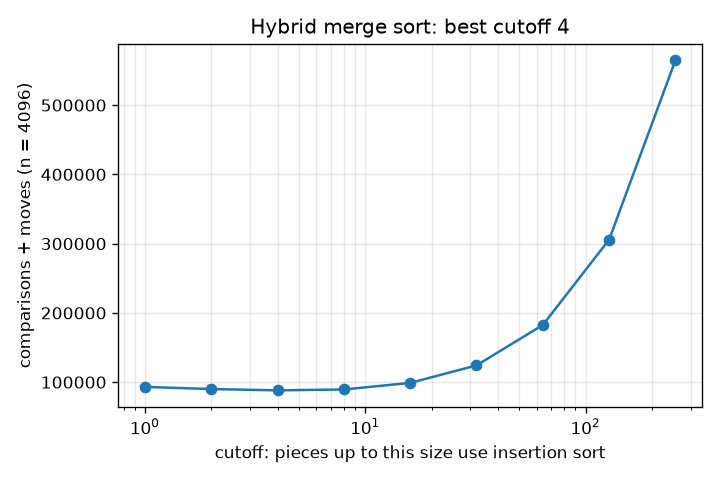
\includegraphics[width=0.85\linewidth]{figures/s03_hybrid_cutoff.png}\\\small Cost of hybrid merge sort against the cutoff for 4096 random items: lowest at a cutoff of 4.\end{center}

\subsection*{E. Worked example}
Quicksort a sorted list of 200 items with three pivot rules: the first item, the median of three, and a random item (seed 0). Compare comparisons and recursion depth with n(n-1)/2.
\begin{enumerate}[nosep]
\item With the first item as pivot, each partition splits off one item. The comparisons are 199 + 198 + ... + 1 = 200 * 199 / 2 = 19,900 and the recursion is 199 levels deep.
\item With the median of three, the pivot is the middle value, so the pieces halve. The code counts 1,534 comparisons (including the 3 used for each pivot choice) and a depth of 7.
\item With a random pivot (seed 0) the code counts 1,625 comparisons and a depth of 16.
\item Compare: 19,900 / 1,534 is about 13 times more comparisons for the first-item pivot, and the gap widens as n grows because n(n-1)/2 grows with the square of n.
\end{enumerate}
\textbf{Answer.} First item: 19,900 comparisons, depth 199. Median of three: 1,534 comparisons, depth 7. Random pivot: 1,625 comparisons, depth 16.

\subsection*{F. Questions}
\begin{enumerate}[nosep]
\item \textbf{Conceptual.} Why is a sorted list the worst case for quicksort with the first item as pivot, and why does that also create a risk of crashing, not just of being slow?
\item \textbf{Numerical.} The comparisons for insertion sort on a reversed list are 4950 for n = 100 and 19,900 for n = 200. Compute the log-log slope between these two points and say what it tells you.
\item \textbf{Graph and simulation interpretation.} On the log-log figure, which lines are parallel, what are their approximate slopes, and what does the gap between the two groups of lines mean?
\item \textbf{Design and optimisation challenge.} Design: 1000 values contain only 10 distinct numbers (many duplicates). Choose among merge sort, quicksort with a first-item pivot and insertion sort, and justify your choice with costs. What does this tell you about the pivot rule?
\end{enumerate}

\section{Real-world mini-project}
\textbf{Choose a sorting method for a nearly sorted data feed.} A feed delivers 2000 records that are already in time order, except that a few records arrived out of place (modelled as random swaps of two positions anywhere in the list). The team wants the method with the lowest cost (comparisons plus moves) and a rule for when to switch. Use \texttt{far\_nearly\_sorted}, \texttt{cost}, \texttt{merge\_sort} and \texttt{crossover\_swaps} from Session 3 to measure insertion sort, merge sort and a hybrid with cutoff 4 for 0, 2, 5, 10, 11, 12, 20, 50 and 100 swaps, and find the number of swaps at which each merge variant first becomes cheaper than insertion sort.

\section{The path ahead}
\begin{enumerate}[nosep]
\item \textbf{Session 4: Run-detecting merge sort.} A natural merge sort that splits the list into runs and merges them, with the same counters.
\item \textbf{Session 5: Three-way quicksort.} A quicksort variant with a three-way partition and the same counters.
\item \textbf{Session 6: A quicksort with no bad input.} A sort that never exceeds twice n log2 n comparisons on any of the five patterns.
\item \textbf{Session 7: Beat the comparison limit.} A counting sort for integers in a small range, measured with the same step counter.
\item \textbf{Session 8: The live race.} An animation that replays several sorts on the same list with live counters.
\end{enumerate}

\section{Answers and hints}

\subsection*{Session 1}
\begin{enumerate}[nosep]
\item \textbf{Conceptual.} Hint: Think about what one swap of two neighbours does to the pairs that are in the wrong order. Solution: A swap of two neighbouring cards changes the order of that one pair only, and when the left card is bigger it fixes that pair. So every swap removes exactly one pair in the wrong order. The row 5 2 4 1 3 starts with 7 such pairs and ends with none, so any method that only swaps neighbours needs exactly 7 swaps. The methods differ only in how many comparisons they waste (10 for bubble sort, 9 for insertion sort).
\item \textbf{Numerical.} Hint: Every pair is in the wrong order. How many pairs are there among 30 cards? Solution: The number of pairs among 30 cards is 30 * 29 / 2 = 435. All of them are in the wrong order, so 435 swaps are needed, and insertion sort compares every card with every card on its left, so there are 435 comparisons as well. Units: counts of steps. Sanity check: a sorted row of 30 needs only 29 comparisons, so 435 is much larger, as it should be for the worst case.
\item \textbf{Graph and simulation interpretation.} Hint: Read the red and blue curves at k = 10. The swap curve is the same for both. Solution: Bubble sort needs 245 comparisons and insertion sort 65, so insertion sort needs 180 fewer. Both need 45 swaps = 10 * 9 / 2, the number of pairs in the wrong order. Insertion sort wins because the part of the row that is already in order is passed by with one comparison per card, while bubble sort still walks through it again and again.
\item \textbf{Design and optimisation challenge.} Hint: Use the pattern 'first 20 reversed' and compare comparisons for the two methods; for the second part count comparisons on a sorted row. Solution: With the first 20 of 30 cards reversed there are 20 * 19 / 2 = 190 pairs in the wrong order, so both methods swap 190 times. Bubble sort needs 390 comparisons and insertion sort 200, so choose insertion sort: about half the work. For an already sorted row both need only 29 comparisons and no swaps, so the choice does not matter. Trade-off: both are fine for 30 cards, but the counts grow with the square of the number of cards, which Session 2 explains.
\end{enumerate}

\subsection*{Session 2}
\begin{enumerate}[nosep]
\item \textbf{Conceptual.} Hint: Compare how the number of steps grows when n grows: n squared versus n log2 n. Solution: Correctness only says what comes out, not how many steps it took. A method with about n(n-1)/2 comparisons needs about 5.0e11 steps for 1,000,000 records; a method with about n log2 n needs about 2.0e7, which is about 25,086 times fewer. On a small list (say 10 items) the difference is a few dozen steps and nobody notices, but because one count grows with n squared and the other with n log2 n, the gap widens as the dataset grows. At 1e9 steps per second that is 500 seconds against 0.02 seconds.
\item \textbf{Numerical.} Hint: Every item must slide past every item before it. Use n(n-1)/2. Solution: For n = 100: 100 * 99 / 2 = 4950 comparisons and 4950 shifts (the code gives exactly 4950 and 4950). For a sorted list each item needs one comparison and no shift, so n - 1 = 99 comparisons and 0 shifts. Units: counts of steps. Sanity check: 4950 is about n squared / 2 = 5000.
\item \textbf{Graph and simulation interpretation.} Hint: Selection sort always scans the whole unsorted part to find the smallest item. Insertion sort stops sliding as soon as the item fits. Solution: Selection sort compares every item with all the items that remain, whatever their order, so it always does n(n-1)/2 comparisons: 499,500 for n = 1000 on any input. Insertion sort stops as soon as the card fits, so on a sorted list it does n - 1 = 999 comparisons and on a reversed list n(n-1)/2 = 499,500. The input order matters for insertion sort and not for selection sort.
\item \textbf{Design and optimisation challenge.} Hint: Count the inversions with \texttt{inversions}, then compare the comparisons of the three sorts on \texttt{nearly\_sorted(1000, 10)}. Solution: The list has only 28 pairs in the wrong order. Insertion sort needs (n - 1) + 28 = 1027 comparisons, merge sort needs 4947, more than 4 times as many, and quick sort with a first-item pivot needs over 400,000 because sorted-looking data is its worst case. Choose insertion sort. Trade-off: if the data were random or reversed, insertion sort would need about n(n-1)/2 = 499,500 steps on reversed input and merge sort would be the better choice. Another trade-off: insertion sort and merge sort are stable, which matters if lines with equal timestamps must keep their order.
\end{enumerate}

\subsection*{Session 3}
\begin{enumerate}[nosep]
\item \textbf{Conceptual.} Hint: What are the sizes of the two pieces after one partition when the pivot is the smallest item? Solution: On sorted input the first item is the smallest, so one piece is empty and the other has n - 1 items. Every level removes just one item, so there are n - 1 levels and n(n-1)/2 comparisons in total (19,900 for 200 items). Recursion depth n - 1 uses one stack frame per level, and Python stops with a RecursionError at its default limit: the checkpoint shows that 1000 sorted items fail with a first-item pivot while the median-of-three pivot succeeds.
\item \textbf{Numerical.} Hint: slope = log2(19,900 / 4950), because n doubled. Solution: 19,900 / 4950 = 4.02, and log2 4.02 = 2.007. The slope is about 2, so the cost grows with the square of n: doubling n multiplies the cost by about 4. Sanity check: n(n-1)/2 is slightly less than n squared / 2, so a slope a little above or below 2 is expected.
\item \textbf{Graph and simulation interpretation.} Hint: Bubble, selection and insertion sort are one group; merge sort and random-pivot quicksort are the other. Use the legend. Solution: Bubble, selection and insertion sort are nearly parallel with slopes between 1.9 and 2.1 (about 2). Merge sort and random-pivot quicksort are nearly parallel with slopes between 1.05 and 1.25 (about 1 plus a little, as 1 + 1/ln n predicts). On a log-log plot a vertical gap is a constant ratio, and because the slopes differ the gap widens: the steeper group costs more and more, relatively, at larger n.
\item \textbf{Design and optimisation challenge.} Hint: Run \texttt{cost} for each method on \texttt{make\_data('duplicates', 1000)}. Solution: Merge sort costs 18,516 (comparisons plus moves) and quicksort with a first-item pivot 57,190, over 3 times more; insertion sort costs hundreds of thousands. Choose merge sort. Quicksort with this partition rule sends all equal items to the same side, so with only 10 distinct values the pieces stop shrinking quickly (an input of 200 identical items costs 19,900 comparisons). A three-way partition fixes this, which is a roadmap milestone. Trade-off: merge sort needs extra memory of order n.
\end{enumerate}

\section{How to join}
Read \texttt{CONTRIBUTING.md} in the repository, then pick an issue labelled \texttt{good first issue}. Repository: \url{https://github.com/KrunalPanchal1995/opensorting}

\end{document}
